\subsection{main()}

Блок-схема на рисунке \ref{fig:main}.

\begin{figure}[pht]
    \center{
        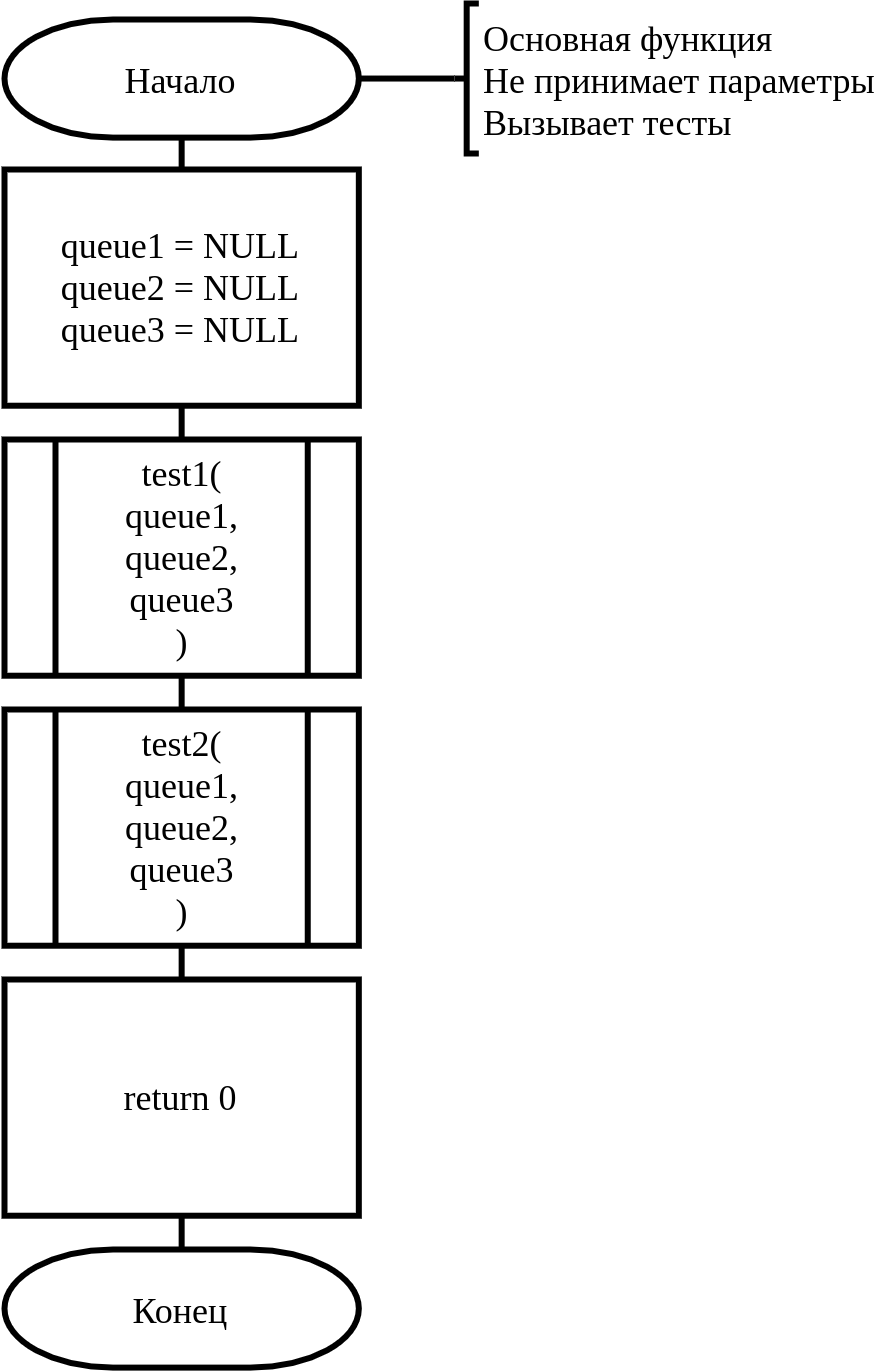
\includegraphics[]{../src/main.png}
    }
    \caption{main()}
    \label{fig:main}
\end{figure}

\lstinputlisting[
    language=C,
    name=main.c
]{../src/main.c}

\lstinputlisting[
    language=C,
    name=main.h
]{../src/main.h}

% = = = = = = = = = = =

\subsection{lab()}

%Блок-схема на рисунке \ref{fig:lab}.

%\begin{figure}[ht]
%    \center{
%        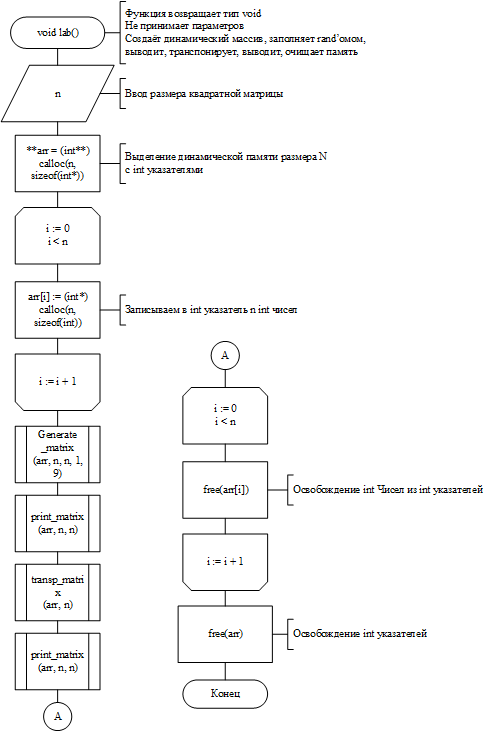
\includegraphics[]{../src/lab/lab.png}
%    }
%    \caption{lab()}
%    \label{fig:lab}
%\end{figure}

\lstinputlisting[
    language=C,
    name=lab.c
]{../src/lab/lab.c}

\lstinputlisting[
    language=C,
    name=main.h
]{../src/lab/lab.h}

% = = = = = = = = = = =

\subsection{add\_element\_to\_node()}

Блок-схема на рисунке \ref{fig:add_element_to_node}.

\begin{figure}[pht]
    \center{
        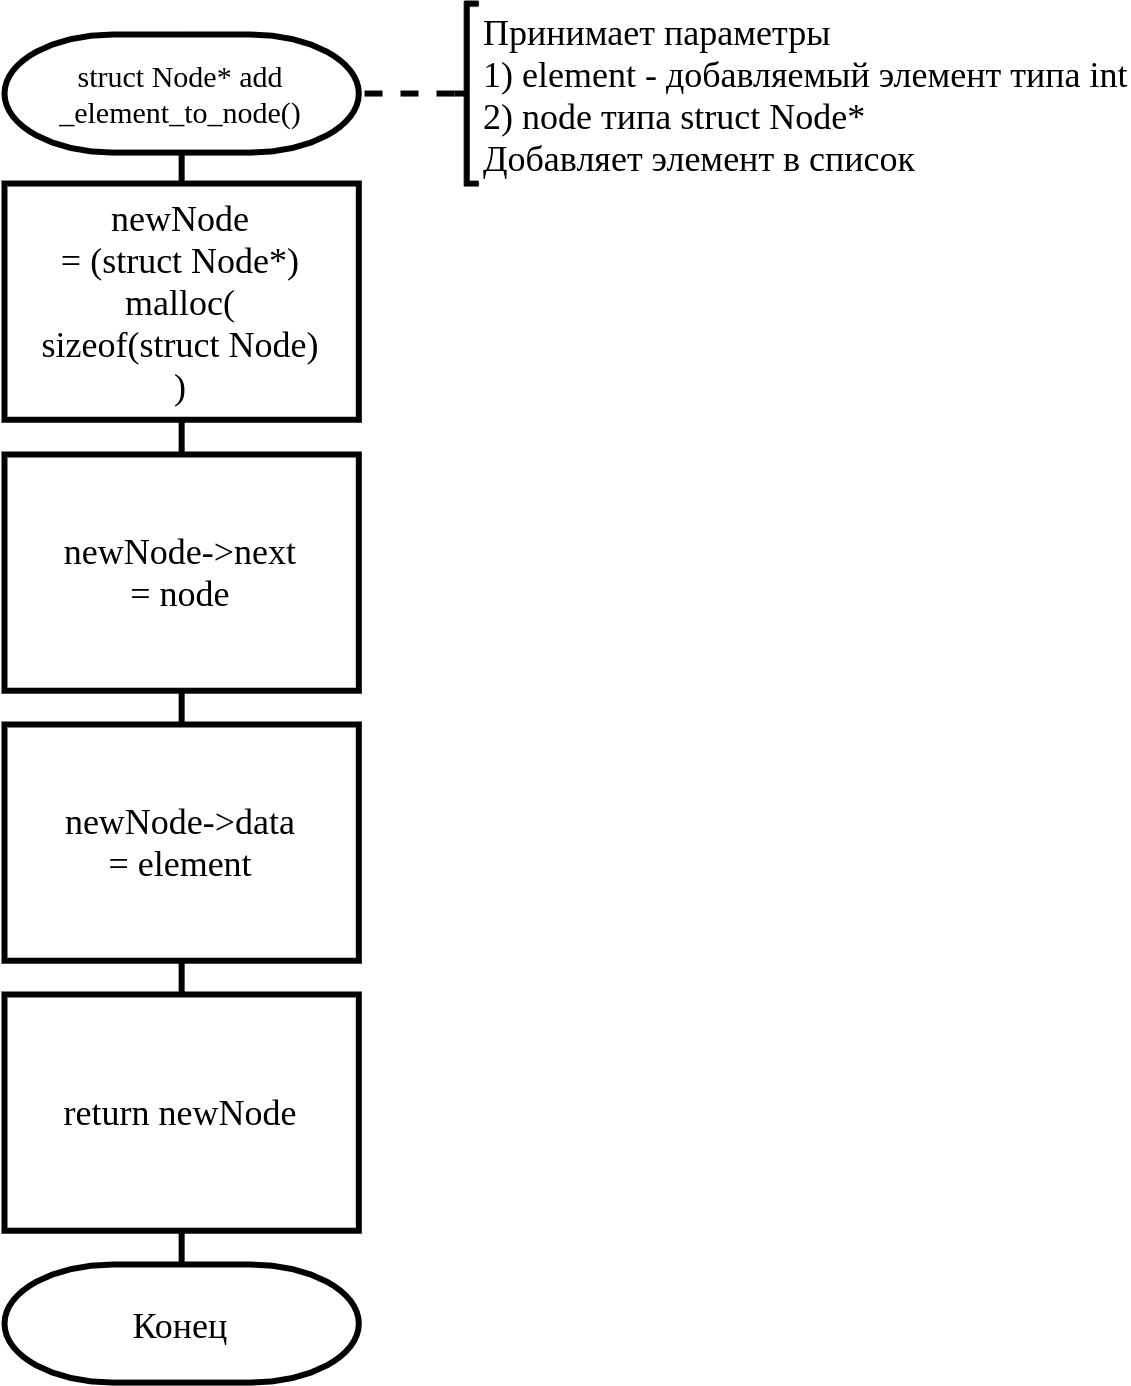
\includegraphics[]{../src/add_element_to_node/add_element_to_node.png}
    }
    \caption{add\_element\_to\_node()}
    \label{fig:add_element_to_node}
\end{figure}

\lstinputlisting[
    language=C,
    name=add\_element\_to\_node.c
]{../src/add_element_to_node/add_element_to_node.c}

\lstinputlisting[
    language=C,
    name=add\_element\_to\_node.h
]{../src/add_element_to_node/add_element_to_node.h}

% = = = = = = = = = = =

\subsection{get\_list\_size()}

Блок-схема на рисунке \ref{fig:get_list_size}.

\begin{figure}[pht]
    \center{
        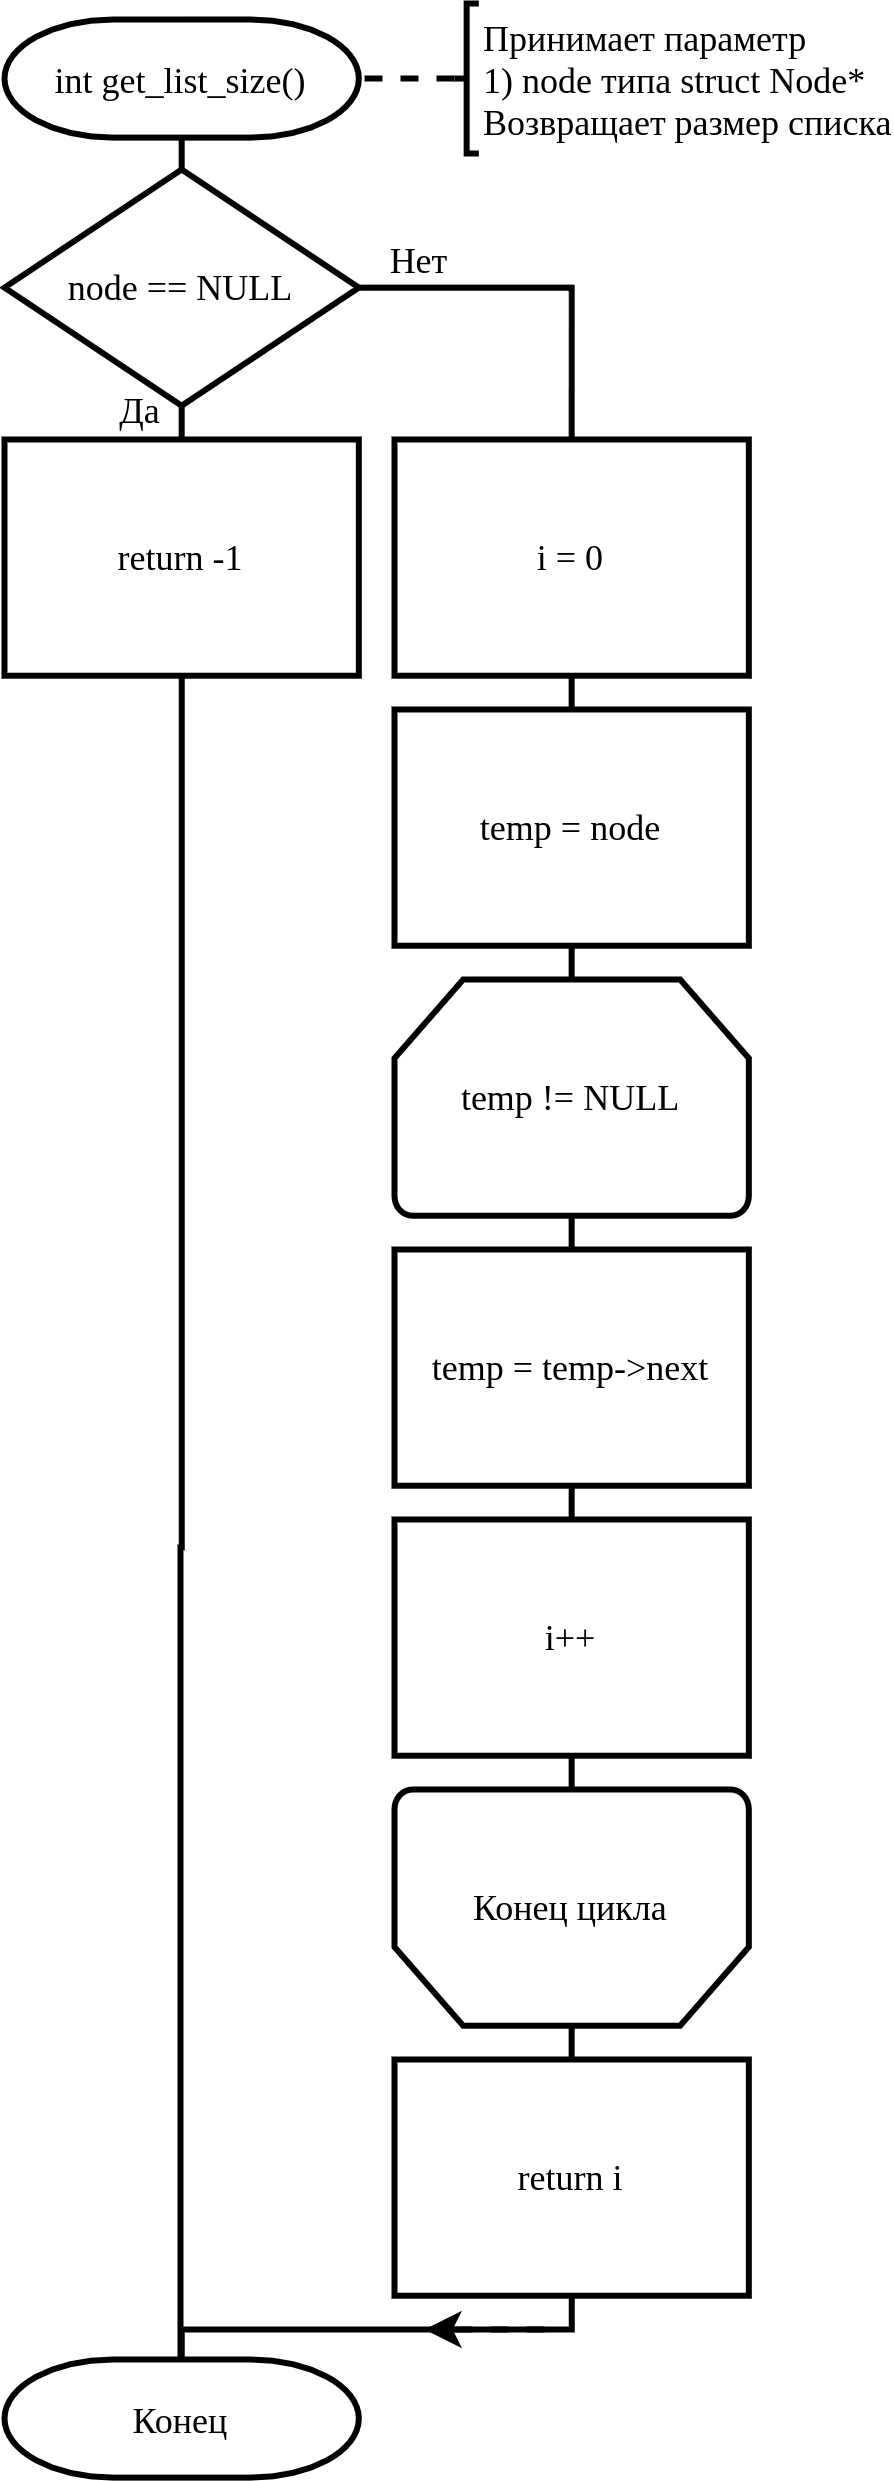
\includegraphics[]{../src/get_list_size/get_list_size.png}
    }
    \caption{get\_list\_size()}
    \label{fig:get_list_size}
\end{figure}

\lstinputlisting[
    language=C,
    name=get\_list\_size.c
]{../src/get_list_size/get_list_size.c}

\lstinputlisting[
    language=C,
    name=get\_list\_size.h
]{../src/get_list_size/get_list_size.h}

% = = = = = = = = = = =

\subsection{print\_list()}

Блок-схема на рисунке \ref{fig:print_list}.

\begin{figure}[pht]
    \center{
        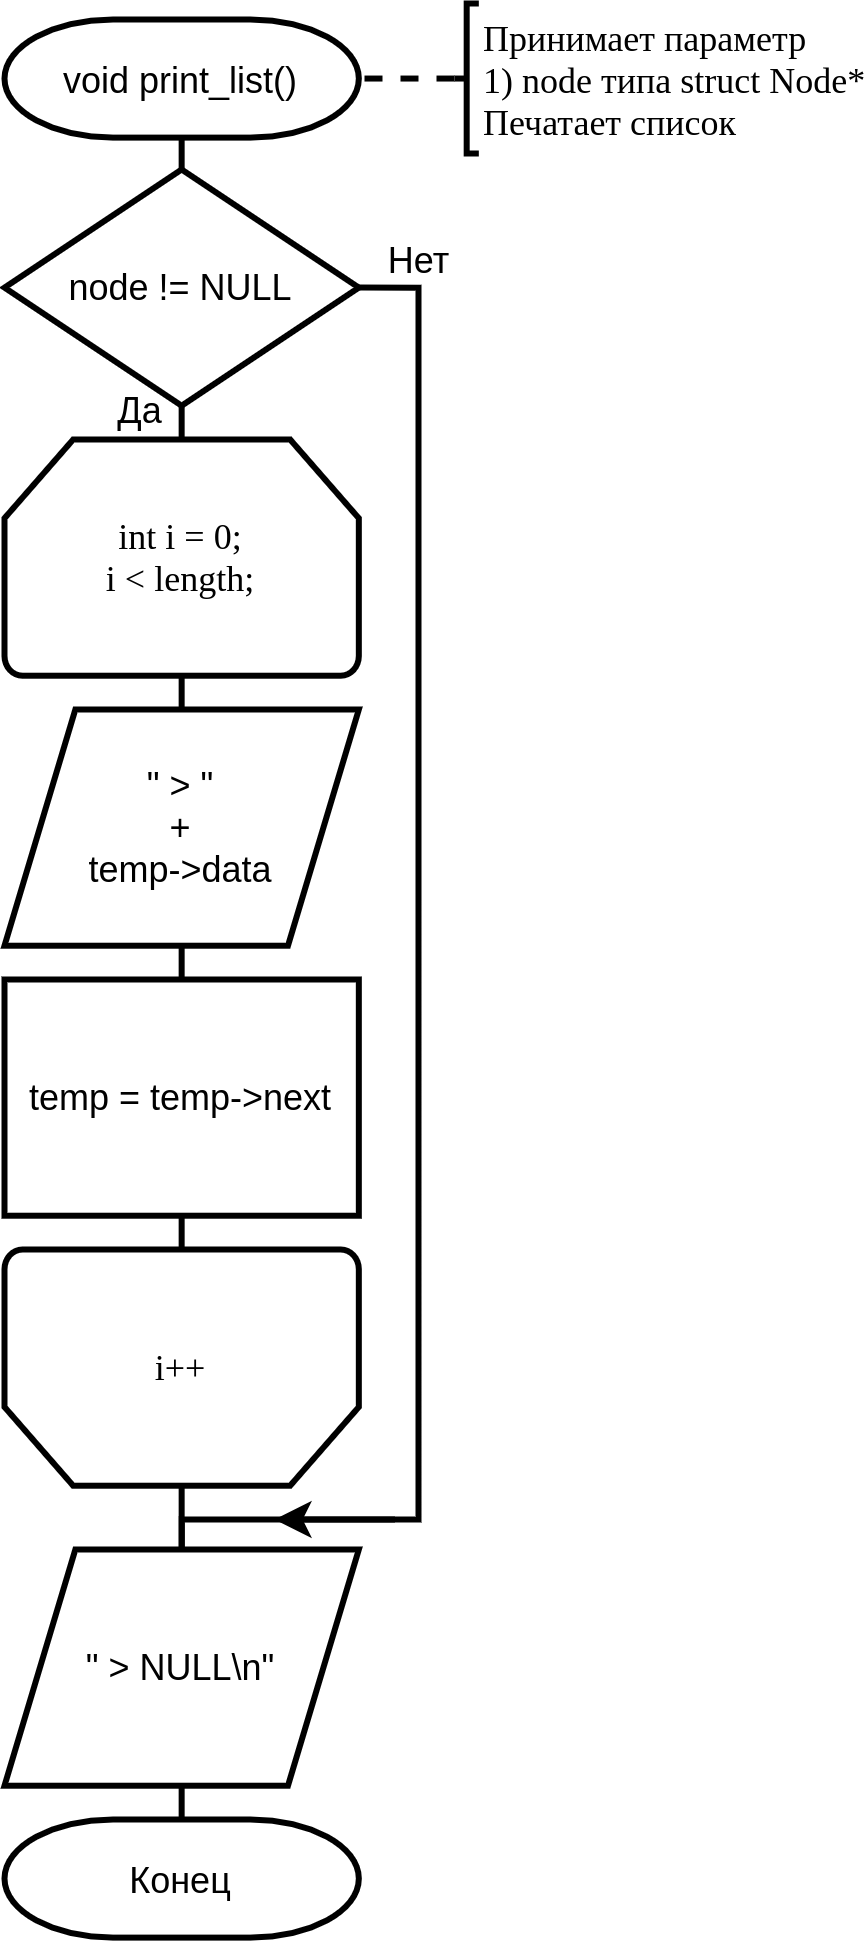
\includegraphics[]{../src/print_list/print_list.png}
    }
    \caption{print\_list()}
    \label{fig:print_list}
\end{figure}

\lstinputlisting[
    language=C,
    name=print\_list.c
]{../src/print_list/print_list.c}

\lstinputlisting[
    language=C,
    name=print\_list.h
]{../src/print_list/print_list.h}

% = = = = = = = = = = =

\subsection{clear\_list()}

Блок-схема на рисунке \ref{fig:clear_list}.

\begin{figure}[pht]
    \center{
        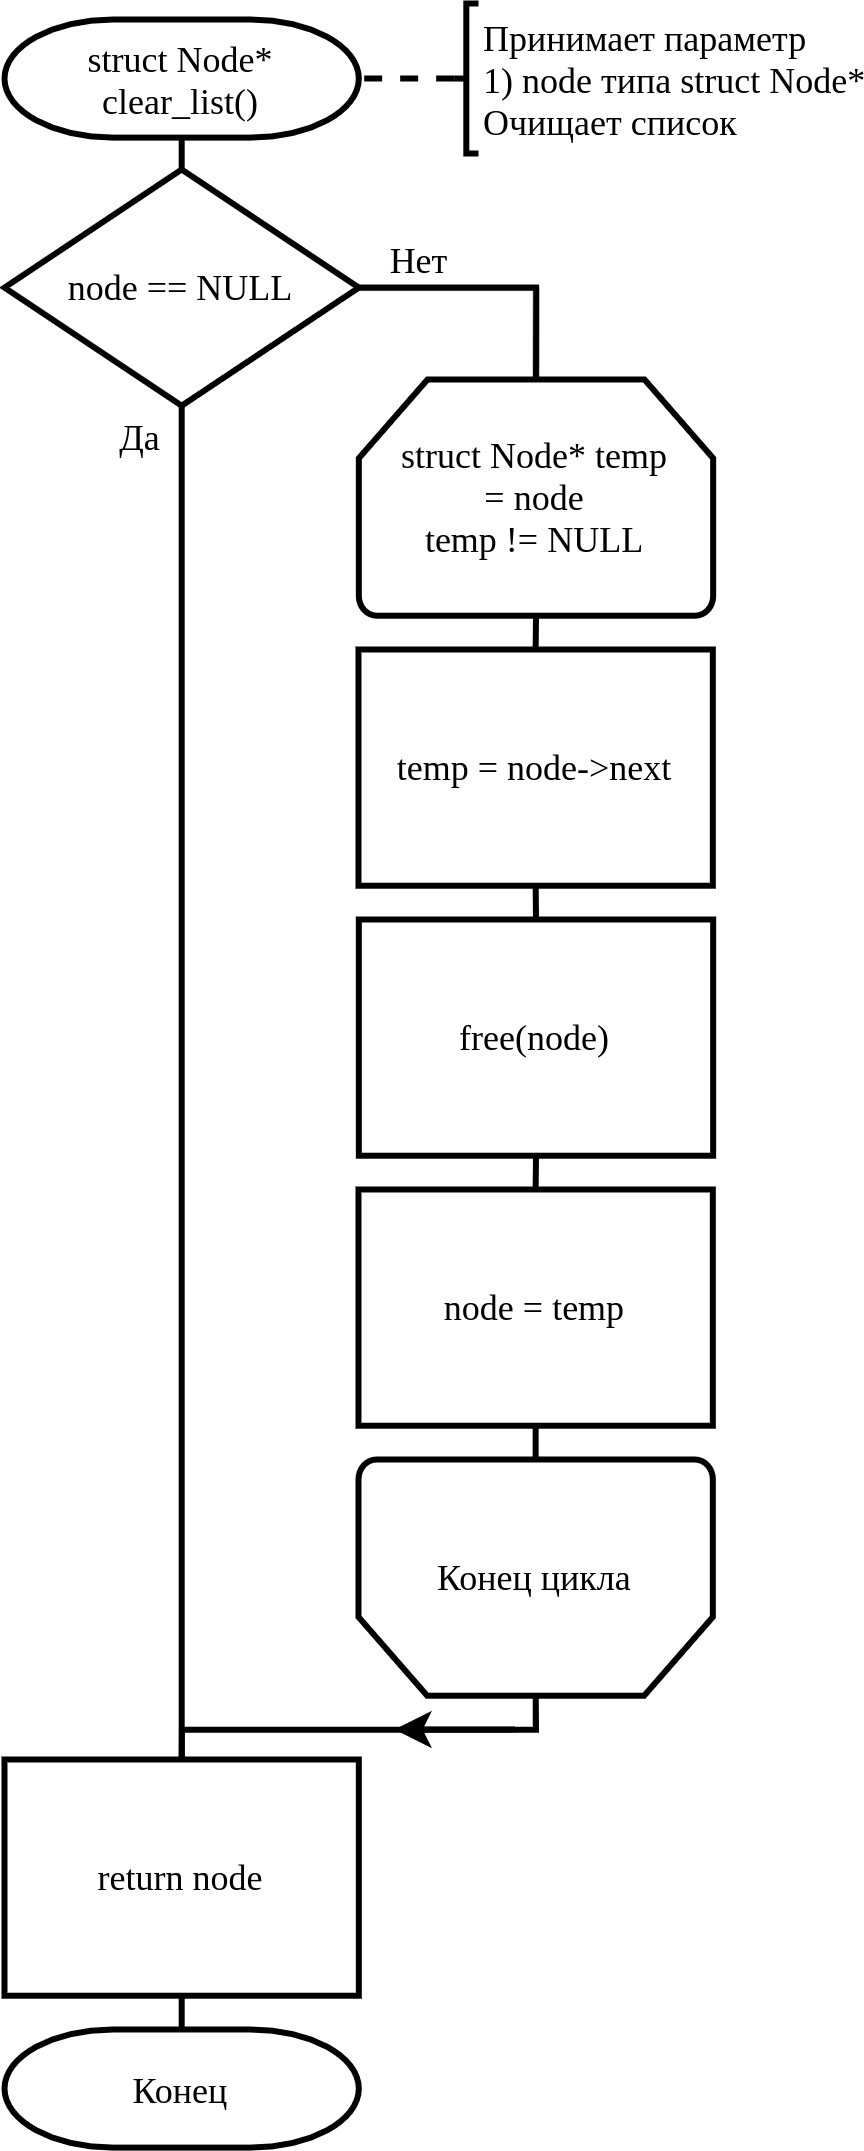
\includegraphics[]{../src/clear_list/clear_list.png}
    }
    \caption{clear\_list()}
    \label{fig:clear_list}
\end{figure}

\lstinputlisting[
    language=C,
    name=clear\_list.c
]{../src/clear_list/clear_list.c}

\lstinputlisting[
    language=C,
    name=clear\_list.h
]{../src/clear_list/clear_list.h}